\documentclass[ruledheader,noindentfirst,anapcustomindent,abntfigtabnum,tocpage=plain]{def_and_cls/abnt}
\usepackage{amsmath, amssymb, amsthm, verbatim, amsfonts, amstext}
%\usepackage[latin1]{inputenc}
\usepackage[brazilian]{babel}
\usepackage[utf8]{inputenc}
\usepackage[T1]{fontenc}
\usepackage{styles/dropping}
\usepackage{graphicx}
\usepackage[hang,small,bf]{caption}
\usepackage[abnt-etal-list=0,abnt-etal-text=it,abnt-and-type=&,abnt-emphasize=bf,abnt-full-initials=yes,alf,bibjustif]{styles/abntcite}
\usepackage{fancyhdr}
\usepackage{makeidx}
\usepackage[none]{hyphenat}
\usepackage{color}
\usepackage{subfig}
\usepackage{styles/algorithms}
\usepackage{algorithmic}
\usepackage{mdwlist}
\usepackage{bm}
\usepackage[titletoc,title]{appendix}
\usepackage{ltxtable}
\usepackage{longtable}
\usepackage{supertabular}
\usepackage{indentfirst}
\usepackage{color}
\usepackage{icomma}

\sloppy


%
%Tradução do pacote Algorithm para portugues
%
\renewcommand{\algorithmicrequire}{\textbf{Entrada:}}
\renewcommand{\algorithmicensure}{\textbf{Saída:}}
\renewcommand{\algorithmicend}{\textbf{fim}}
\renewcommand{\algorithmicif}{\textbf{se}}
\renewcommand{\algorithmicthen}{\textbf{então}}
\renewcommand{\algorithmicelse}{\textbf{senão}}
\renewcommand{\algorithmicelsif}{\algorithmicelse \, \algorithmicif}
\renewcommand{\algorithmicendif}{\algorithmicend \, \algorithmicif}
\renewcommand{\algorithmicfor}{\textbf{para}}
\renewcommand{\algorithmicforall}{\textbf{para todo}}
\renewcommand{\algorithmicdo}{\textbf{fazer}}
\renewcommand{\algorithmicendfor}{\algorithmicend \, \algorithmicfor}
\renewcommand{\algorithmicwhile}{\textbf{enquanto}}
\renewcommand{\algorithmicendwhile}{\algorithmicend \, \algorithmicwhile}
\renewcommand{\algorithmicloop}{\textbf{laço}}
\renewcommand{\algorithmicendloop}{\algorithmicend \, \algorithmicloop}
\renewcommand{\algorithmicrepeat}{\textbf{repetir}}
\renewcommand{\algorithmicuntil}{\textbf{até}}
\renewcommand{\algorithmiccomment}[1]{\{#1\}}
\renewcommand{\listalgorithmname}{Lista de Algoritmos}
\floatname{algorithm}{Algoritmo}
%%%%%%%%%%%%%%%%%%%%%%%%%%%%%%%%%%%%%%%%%%%%%%%%%%%%%%%%%%%%%%%%%%%%%%%%%%%%%%%%%%%

\makeindex

%%%% O arquivo modelosCAP.tex possui as definições para ciação do estilo de capítulo (fonte de título, barras horizontais, etc.)
% ele não gera texto de saída, é um arquivo de configuração somente
%
%Estilo de formatação de capítulos

\makeatletter
\newcommand{\thechapterwords}
{ \ifcase \thechapter\or 1\or 2\or 3\or 4\or 5\or6\or 7\or 8\or 9\or 10\or 11\fi}

\def\@makechapterhead#1{%
\vspace*{10\p@}%
{\parindent \z@  \reset@font

\scshape \@chapapp{} \thechapterwords
\quad %
\par\nobreak
\vspace*{10\p@}%
\interlinepenalty\@M
\hrule
\vspace*{10\p@}%
\Huge \bfseries #1\par\nobreak
\par
\vspace*{10\p@}%
\hrule
\vskip 40\p@
}}
\def\@makeschapterhead#1{%
\vspace*{10\p@}%
{\parindent \z@ \centering \reset@font
\par\nobreak
\vspace*{10\p@}%
\interlinepenalty\@M
\hrule
\vspace*{10\p@}%
\Huge \bfseries #1\par\nobreak
\par
\vspace*{10\p@}%
\hrule
\vskip 40\p@
%\vskip 100\p@
}}
%%%%%%%%%%%%%%%%%%%%%%%%%%%%%%%%%%%%%%%%%%%%%%%FIM DO PREAMBULO%%%%%%%%%%%%%%%%%%%%%%%%%%%%%%%%%%%%%%%%%%%%%%%%%%%%%%%%%%%%%%%%%%


\begin{document}

%%%%% IMPORTANTE: ALTERA O TEXTO ENTRE ARIAL E TIMES NEW ROMAN (ALTERNAR OS COMENTÁRIOS)
%
%%%%%%%%%%%%%%%%%%%%%PARA UTILIZAR ARIAL%%%%%%%%%%%%%%%%%%%%%%%
%
\fontfamily{phv}                    %fonte Arial
\renewcommand{\rmdefault}{phv}      %
%
%%%%%%%%%%%%%%%%%%%%%PARA UTILIZAR TIMES%%%%%%%%%%%%%%%%%%%%%%%
%
%\fontfamily{ptm}               %fonte Times
%\renewcommand{\rmdefault}{ptm} %
%
%%%%%%%%%%%%%%%%%%%%%%%%%%%%%%%%%%%%%%%%%%%%%%%%%%%%%%%%%%%%%%%

%%%%%%%%%%%%%Arquivos .tex com os elementos pré-textuais
%
\thispagestyle{empty}

\vfill
 \begin{center}
    \begin{figure}[t]
     \centering
            
\includegraphics[width=5cm]{figures/IF_logo.eps}\\[-0.1in]
     \end{figure}

    {\large\bfseries INSTITUTO FEDERAL DE EDUCAÇÃO, CIÊNCIA E TECNOLOGIA DO CEARA} \\
    {\large\bfseries PRÓ-REITORIA DE ENSINO} \\
    {\large\bfseries COORDENADORIA DE TELEMÁTICA DO CAMPUS MARACANAÚ}  \\ 
    {\large\bfseries BACHARELADO EM CIÊNCIA DA COMPUTAÇÃO}  \\ 

    \vspace*{1in}
    \begin{large} \bfseries FELIPE MARCEL DE QUEIROZ SANTOS \end{large}\\[0.4in]

    \vspace*{4cm}
    \noindent \\
    \large\bfseries{TÍTULO DO TRABALHO} \\
    \vfill
    \large\bfseries{ MARACANAÚ \\ 2015}
\end{center}

\normalsize
%\begin{titlepage}
\vfill
\begin{center}

    {\large FELIPE MARCEL DE QUEIROZ SANTOS\\}
    \vspace{2cm}
    {\Large \textsc{TiTULO DO TRABALHO}\\}
    \vspace{1cm}
    \hspace{.45\linewidth}
    \begin{minipage}{.50\linewidth}

            Monografia submetida à Coordenadoria de Telemática e à Coordenadoria do Curso de Bacharelado 
            em Ciência da Computação do Instituto Federal do Ceará - Campus Maracanaú, como requisito 
            parcial para obtenção do grau de Bacharel em Ciência da Computação.

            \vspace{0.5 cm}

            Área de pesquisa: Aprendizagem de Máquina

            \vspace{0.5 cm}

            Orientador:D.r AMAURI HOLANDA SOUZA JUNIOR
    
    \end{minipage}

    \vspace{2cm}
    \vfill
    {\large Maracanaú\\ 2015}
\end{center}

\end{titlepage}
%\begin{folhadeaprovacao}
\setlength{\ABNTsignthickness}{0.2pt}
\setlength{\ABNTsignskip}{1.7cm}

\begin{center}

\includegraphics[width=2.5cm]{figures/brasao_republica.eps}\\
            {ESCOLA POLITÉCNICA DA USP} \\

    \vspace{1.5cm}
                                    {NOME DO ALUNO}\\
    \bfseries{}
\end{center}

Esta Monografia foi julgada adequada para a obtenção do Grau de Bacharel em Ciência da Computação, sendo aprovada pela Coordenadoria de Telemática e pela Coordenadoria do curso de Bacharelado em Ciência da Computação do Campus Maracanaú do Instituto Federal de Educação, Ciência e Tecnologia do Ceará e pela banca examinadora:

    \vspace{0.15cm}
    \assinatura{Orientador: Prof. Dr. Amauri \\ Instituto Federal do Ceará - IFCE}
    \assinatura{Prof. Dr. Huguinho \\ Instituto Federal do Ceará - IFCE}
    \assinatura{Prof. Dr. Zezinho \\ Instituto Federal do Ceará - IFCE}
    \assinatura{Prof. Dr. Luizinho \\ Instituto Federal do Ceará - IFCE}
    \vspace{0.15cm}%\vfill

    \begin{center}
        Fortaleza, 06 de Abril de 2013
    \end{center}
\end{folhadeaprovacao}
%\vspace*{15cm}

\hfill Dedico este trabalho ...\\
%\chapter*{Agradecimentos}
%%\thispagestyle{empty}


\begin{flushright}
\begin{minipage}[r]{10cm}
\vspace{18cm}
``A mente que se abre a uma nova idéia jamais voltará ao seu tamanho original''.
\begin{flushright}
Albert Einstein
\end{flushright}
\end{minipage}
\end{flushright}
\pagestyle{plain}%%%%% Utilizar ESTILO PLAIN AQUI%%%%%%%
%\chapter*{Resumo}

\noindent Este trabalho apresenta...
%\chapter*{Abstract}


\noindent This work presents...

%%%Comandos para criação automática das listas
%
\tableofcontents


%%%%%%%%%%%%%%%%%%%%%%%%%%%%%%%%%%%%%%%%%%%%%%%%%%%%%%%%%%%%%%%%%%%%

%Capítulos passam a ter páginas numeradas
%
\pagestyle{fancy}

%resseta os contadores de capítulo e seção
%
\renewcommand{\chaptermark}[1]{\markboth{#1}{}}
\renewcommand{\sectionmark}[1]{\markright{\thesection\ #1}}

%%%%%%%%%%%%%%NÃO LEMBRO O QUE FAZ, APARENTEMENTE NADA, TESTAR DEPOIS
%\fancyhf{}%
%\fancyhead[RO,LE]{\large\slshape\thepage}%
%\fancyhead[CE]{\large\slshape\leftmark}%
%\fancyhead[CO]{\large\slshape\rightmark}%


%%% Outros arquivos .tex. É acoselhável utilizar vários arquivos, pelo menos um por capítulo

\chapter{Introdução}\label{CAP:introducao}
%\thispagestyle{empty}

% Este documento consiste de um modelo basico para a producao de documentos academicos, seguindo as normas ABNT. 

% Nao e abordado o estudo do LaTex neste template. Sugerimos a leitura do texto em \citeonline{Oetiker:1995}. O uso do LaTex e aconselhavel devido a sua qualidade grafica, facil referenciacao, criacao de listas, indices, referencias bibliograficas e escrita matematica profissional. Porem, nao e obrigatorio o uso deste template, apenas as orientacoes de formatação segundo as normas ABNT devem ser obrigatoriamente seguidas.

% Uma observação em particular é a de que, no pacote ABNTex, as referências diretas devem utilizar o comando ``citeonline''. Referências indiretas utilizam o comando ``cite''.

% Exemplo de citacao direta: Uma otima fonte de estudo para compreender o LaTex e apresentada por \citeonline{Oetiker:1995}. 

% Exemplo de citação indireta: Existem boas fontes de pesquisa para entendimento do LaTex \cite{Oetiker:1995}, estas incluem documentação online disponível na web.
blablabla

\section{Objetivos}


 
\section{Diferenças UML e SysML}




\sectioan{Uso}


\section{História}

Com o intuito de elaborar uma linguagem unificada de propósito geral para engenharia de sistemas, diante das limitações da UML (Unified Modeling Language) a SysML foi criada pelo Object Management Group (OMG) em conjunto com o International Council on Systems Engineering (INCOSE). 

Em 2003, foram publicados os requisitos de uma linguagem de modelagem que servisse para Engenharia de Sistemas, criando-se, em seguida, um grupo de trabalho composto por representantes da indústria e produtores de ferramentas CASE chamado SysML Partners. Esse grupo ficou responsável por desenvolver a linguagem respeitando os requisitos estabelecidos. 

Em 2004 foi publicada a versão draft da SysML e em 2005 a versão SysML 1.0. A versão formal pública SysML OMG v 1.2 foi publicada pela  OMG em Junho de 2010. Desde então a linguagem vem se tornando cada vez disseminada e aceita pela comunidade se mostrando adequada para as demandas de Engenharia de Sistemas.

Assim surgiu a SysML, como uma extensão da UML V2 que expande a proposta de programação orientada a objetos possibilitando a representação de requisitos do sistema, componentes que não são de softwares, equações, fluxos contínuos e alocações.


\noindent \textbf{Capitulo \ref{CAP2}}: descricao...

\noindent \textbf{Capitulo \ref{CAP3}}: descricaoo...

\noindent \textbf{Capitulo \ref{CAP4}}: descricao...

\noindent \textbf{Capitulo \ref{CAP5}}: descricao...
\chapter{Diagramas}
\label{CAP2}

Neste capítulo são descritos em algum detalhe os diferentes diagramas do SysML. 


\section{Diagrama de Definição de Bloco}
\subsubsection{O que é diagrama de definição de blocos}

O diagrama de definições de bloco é baseado no diagrama de classes da UML com o adicional de algumas restrições e extensões definidas dentro da SysML. Sendo o diagrama mais usado dentro dessa. Sua função é modelar os aspectos estruturais, através de blocos, de um sistema, mostrando os elementos físicos, relacionamentos, fluxos e hierarquias.

\subsubsection{Estrutura dos diagramas de definição de blocos}

Com a proposta de mostrar diferentes elementos do fluxo e suas relações a figura abaixo mostra o diagrama de definição de blocos de uma ACME câmera, com os símbolos mais comuns do diagrama de blocos.

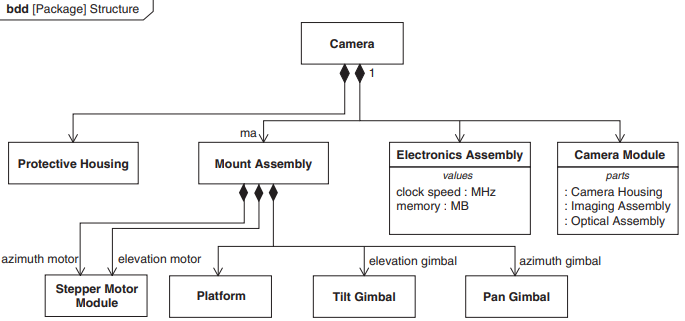
\includegraphics[width=\textwidth,height=\textheight,keepaspectratio]{figures/diagrama de blocos.PNG}

\paragraph{}
 \textbf{Elementos físicos} 
 
 
Os elementos físicos são graficamente representados por blocos. Eles podem ser hardwares, softwares, pessoas ou qualquer outra entidade lógica ou conceitual. 

O nome do bloco aparece em seu topo em negrito, enquanto as outras propriedades tem seus compartimentos abaixo em letra minúscula, itálico e espaço entre as palavras. Essas propriedades podem ser de três diferentes tipos. 

Uma delas é propriedade de parte, que decompõem o bloco nos elementos que os constituem, por exemplo, no diagrama acima, dentro do bloco de "Camera Module"  tem-se as partes "Camera Housing", "Imaging Assembly"  e "Optical Assembly".

Outra é a propriedade de referência, que referencia partes de outro bloco indicando em que partes o blocos conectados se relacionam. 

Por fim, pode-se ter também a propriedade de valor, responsável por descrever as características quantificáveis do bloco, no diagrama acima, o bloco "Eletronics Assembly"  tem as propriedades de valor "clock speed"  em MHz e "memory"  em MB.

\paragraph{}
 \textbf{Relacionamento entre blocos} 
 
O relacionamento entre blocos indica como os blocos se relacionam, de maneira geral ele é representado com uma linha simples com elementos nas pontas, que irá indicar qual a relação exata entre eles. Existem quatro tipos diferentes de relação que podem ser representados no diagrama de blocos.

A conexão de composição é representada graficamente por um losango preenchido conectado em um bloco maior com um traço embaixo ligando a outros blocos, é utilizado para indicar que o bloco maior possui outros elementos definindo assim uma propriedade de parte no bloco maior. Existe a possibilidade de se colocar uma seta na outra parte, neste caso faz alusão a alguma propriedade referência. A propriedade de parte é escrita no diagrama em cima do bloco de chegada quando o nome do bloco em si não oferece informações suficientes, enquanto a propriedade de referência é escrita em cima do bloco de partida. No diagrama acima, o bloco "Mount Assembly", por exemplo esta ligado desta maneira aos blocos "Stepper Motor Module" duas vezes, em relação as partes "azimuth motor" e ao "elevation motor", já na relação entre o bloco "Camera" e "Eletronics Assembly" não foi necessário indicar o nome da parte de referência, uma vez que o próprio bloco descreve bem o ponto de conexão.

A conexão de referência é representada graficamente por um losangolo vazio em uma ponta ligado por uma seta a outros elementos. Ela é utilizada para indicar que um bloco referencia o outro, quando existe uma referencia apenas de um lado da relação é utilizada uma seta no bloco que contém a propriedade de referência, já se ambos blocos se referenciam entre si não são utilizadas setas. As referencias, quando não indicadas como propriedades do bloco, são escritas em cima do bloco, da mesma maneira que as propriedades de parte na conexão de composição. 

A conexão por associação 



\section{Diagrama de Definição de Blocos Internos}
\section{Diagrama de Definição de Parâmetros}
\section{Diagrama de Definição de Pacote}
\section{Diagrama de Definição de Requisitos}
\section{Diagramas Comuns ao UML}
As seções a seguir descrevem alguns dos diagramas comuns ao UML.

\subsection{Diagrama de Máquina de Estados}
Nesta seção será descrito o diagrama de máquina de estados, presente no SysML e também no UML. Ele é .......

\subsubsection{O que é o diagrama de máquinas de estados}
Texto

\subsubsection{Estrutura dos diagramas de máquinas de estado}
Texto

\subsubsection{Onde são utilizados com frequência}
Texto

\subsection{Diagrama de Sequência}
Nesta seção será descrito o diagrama de sequência, presente no SysML e também no UML. Ele é .......

\subsubsection{O que é o diagrama de sequência}
Texto

\subsubsection{Estrutura dos diagramas de sequência}
Texto

\subsubsection{Onde são utilizados com frequência}
Texto

\subsection{Diagrama de Casos de Uso}
Esta seção descreve mais um dos diagramas do SysML que também existem no UML. Os diagramas de caso de uso são centrais no processo de desenvolvimento de sistemas, e normalmente são desenvolvidos no início desse processo.

\subsubsection{O que são casos de uso}

Casos de uso descrevem a funcionalidade de um sistema em termos de como ele é utilizado para atingir os objetivos de seus usuários. Os usuários de um sistema são descritos como atores, que podem representar sistemas externos ou humanos que interagem com o sistema cujo caso de uso está sendo descrito.

As relações entre o sistema, seus atores e os casos de uso é, então, descrita no diagrama de casos de uso.
Casos de uso podem também ser elaborados com descrições detalhadas de seu comportamento, fazendo uso de diagramas de Atividade, de Sequência, de Contexto ou de máquinas de estado.

Um caso de uso tipicamente cobre vários cenários, que são representados como caminhos através do caso de uso, que acontecem cada um numa circunstância diferente.

\subsubsection{Estrutura dos diagramas de casos de uso}
Os diagramas de caso de uso descrevem um conjunto de atores e de casos de uso e o relacionamento entre eles.

A figura abaixo mostra um exemplo de diagrama com seus principais elementos: um sistema (Surveillance System), atores (Operator, Intruder e Emergency Services) e um caso de uso (Monitor Environment), além das multiplicidades dos atores e do caso de uso. Multiplicidades implícitas são 0…1. Mais sobre multiplicidades a seguir.

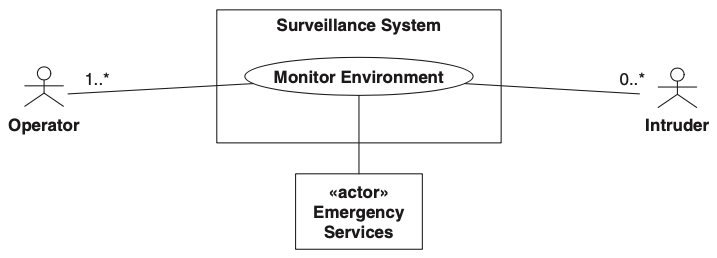
\includegraphics[width=\textwidth,height=\textheight,keepaspectratio]{figures/diagrama-caso-de-uso-1.png}

Um ator é sempre externo ao sistema. Ser interno ou externo a um sistema depende do sistema que estiver sendo avaliado. Uma pessoa pode ser um ator de um caso de uso ao utilizar certo sistema, mas, quando um outro sistema de que ela faz parte tiver seus casos de uso descritos por diagramas de caso de uso, essa pessoa deixa de ser um ator e passa a ser parte do sistema sob análise.

O pacote completo do diagrama de caso de uso pode conter diagramas que descrevem mais detalhadamente cada um dos atores envolvidos no caso de uso, como no exemplo a seguir.

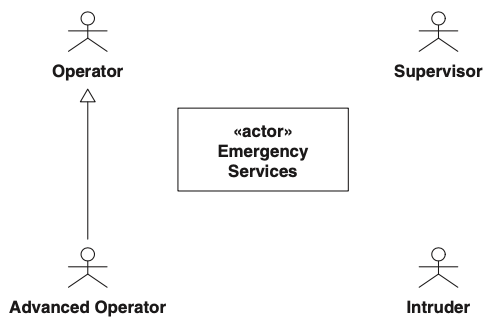
\includegraphics[width=\textwidth,height=\textheight,keepaspectratio]{figures/diagrama-caso-de-uso-2.png}

A relação entre atores e casos de uso tem características como multiplicidade. A multiplicidade do caso de uso representa com quantas instâncias do caso de uso cada ator interage por vez. A multiplicidade do lado do ator representa quantos atores podem interagir com aquele caso de uso por vez.

O diagrama exemplificado acima mostra apenas um caso de uso. Contudo, os diagramas de casos de uso podem mostrar mais de um caso de uso, suas relações, e todos os atores envolvidos. O exemplo abaixo mostra como os casos de uso interagem entre si utilizando as palavras-chave \textit{extend} e \textit{include}.

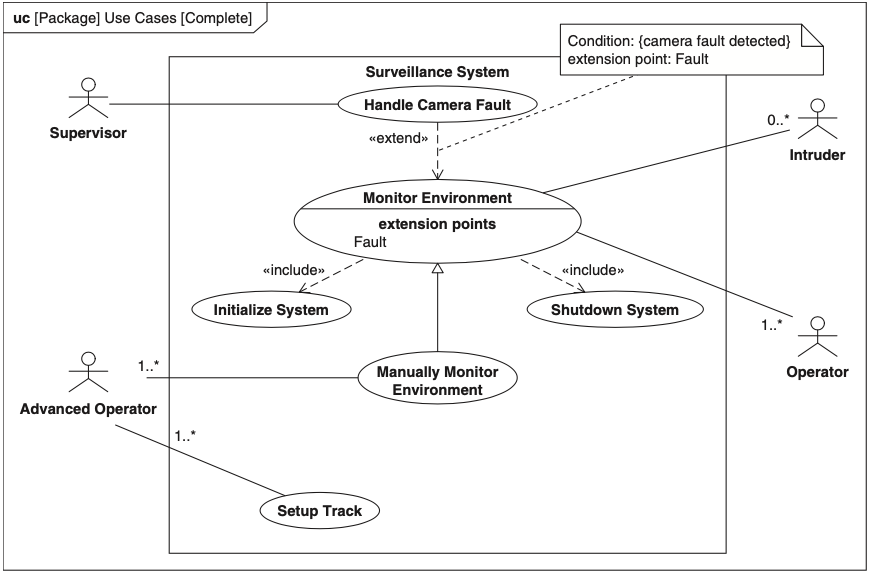
\includegraphics[width=\textwidth,height=\textheight,keepaspectratio]{figures/diagrama-caso-de-uso-3.png}

\begin{itemize}
\item \textit{include}: indica que um caso de uso utiliza a funcionalidade do caso de uso ao final da seta em algum momento do seu fluxo de trabalho. Assim, os atores que interagem com o caso de uso na base da seta também interagem com o caso de uso incluído.
\item \textit{extend}: indica casos de uso que realizam alguma extensão do fluxo de trabalho do caso de uso na base da seta. Trata-se de funcionalidades que não são consideradas parte do caso de uso base, diferentemente da relação de inclusão.
\end{itemize}

Casos de uso também podem ser descritos de maneira textual, utilizando as palavras-chave a seguir:
\begin{itemize}
\item \textbf{Pré-Condições}: Condções necessárias para o caso de uso iniciar.
\item \textbf{Pós-Condições}: Condições necessárias após o fim da execução do caso de uso.
\item \textbf{Fluxo Primário}: Fluxo de trabalho mais frequente do caso de uso
\item \textbf{Fluxos alternativos ou de exceção}: podem existir vários, e mostram o que acontece em situações menos frequentes ou em que o sistema apresenta algum erro.
\end{itemize}

\subsubsection{Onde são utilizados com frequência}

Casos de uso são a forma principal de se descrever os requisitos para um novo software sob desenvolvimento. Eles especificam o comportamento esperado do sistema.

Assim, diagramas de caso de uso são normalmente desenvolvidos nos estágios iniciais do desenvolvimento de um sistema, e, comumente, tem o propósito de especificar o contexto do sistema, capturar os requisitos do sistema, validar a arquitetura do sistema e gerar casos de teste.

Os diagramas normalmente são desenvolvidos conjuntamente por desenvolvedores de sistemas e por \textit{experts} de domínio, nas fases iniciais de levantamento de requisitos de um sistema. 

\subsection{Diagrama de Atividade}



%%%% Estilo de citação ABNT e arquivo de bibitens (mybibliography.bib)
\bibliographystyle{abnt-alf}
\bibliography{mybibliography}

\apendice
\chapter{Título do Apêndice}
\label{Apx:A}




\chapter{Exemplo do pacote Algorithm}
\label{Apx:B}


\begin{algorithm}[!h]
\caption{Estimador ML otimizado.}\label{Alg:MAXVER}
\begin{algorithmic}[1]
\STATE Inicializar o contador: $j\leftarrow 1$;%
\STATE Fixar o limiar de variação das estimativas: $e_{\mathrm{out}}\leftarrow 10^{-4}$;%
\STATE Fixar o número máximo de iterações: $N\leftarrow 1000$;%
\STATE Computar o ponto inicial: $\hat \gamma(0)$;%
\STATE Determinar o limiar inicial: $e_1 \leftarrow1000$;%
\STATE Estabelecer o valor inicial de $\alpha$: $\hat \alpha(0) \leftarrow -10^{-6}$;%
\WHILE{ $e_j \geq e_{\mathrm{out}}$ e $ j\leq M$}
    \STATE Solucionar $\hat \alpha_j\leftarrow {\arg \max}_{\alpha}\;{l_1(\alpha; \gamma_{j-1},\mathbf{z},n)}$;%
    \STATE Solucionar $\hat \gamma_j\leftarrow {\arg \max}_{\gamma}\;{l_2(\gamma; \alpha_j,\mathbf{z},n)}$;%
    \STATE $j\leftarrow j+1$
    \STATE Computar o critério de convergência: $e_j$;%
\ENDWHILE
\end{algorithmic}
\end{algorithm}


\end{document}